\documentclass[tikz,border=10pt]{standalone}
% No extra TikZ libraries needed: all coordinates are precomputed.
\begin{document}
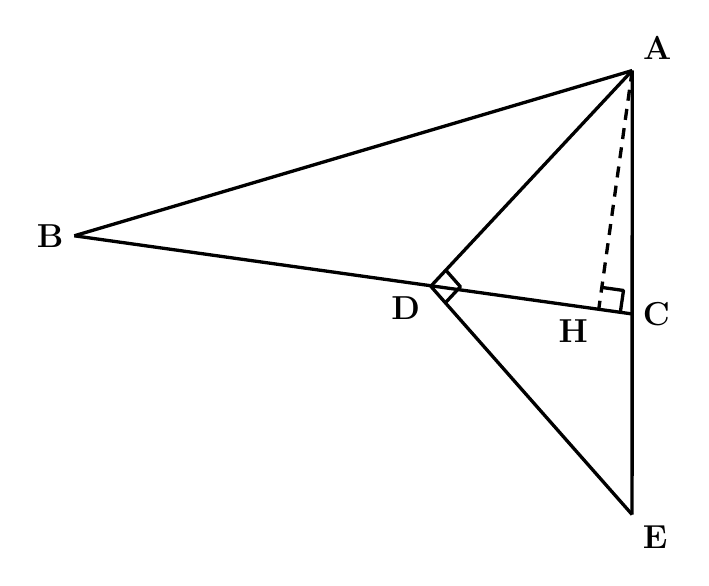
\begin{tikzpicture}[line width=1.2pt, line join=round, font=\fontsize{12}{14.4}\selectfont]
  % Named points (scale s = 0.014981 cm/px, y flipped, centred on ink bbox)
  \coordinate (A) at (3.538005804762978,2.8183200128814754);
  \coordinate (B) at (-3.5468588807971457,0.7200066945911826);
  \coordinate (C) at (3.5352904571347707,-0.27250747123498953);
  \coordinate (D) at (0.98,0.079);
  \coordinate (E) at (3.536349937609236,-2.820000307482368);
  \coordinate (H) at (3.1132126812901615,-0.21281892875530015);

  % Solid segments
  \draw (B) -- (A);
  \draw (B) -- (C);   % passes through D
  \draw (A) -- (D);
  \draw (D) -- (E);
  \draw (A) -- (E);   % passes through C

  % Dashed segment A-H
  \draw[dash pattern=on 4pt off 3pt] (A) -- (H);

  % Right-angle mark at H (between HA and HC)
  \draw (3.152821052380861,0.06423606081598995) -- (3.427176272760402,0.02551705922450792) -- (3.3872950224638654,-0.251473998349438);

  % Right-angle mark at D (between DA and DE)
  \draw (1.1709087190647764,0.28308529981259584) -- (1.3559230009354746,0.07309782414204312) -- (1.1650142818706979,-0.1309874756705528);

  % Labels (bold math to match original weight; vertex dots removed)
  \node[above right] at (A) {$\mathbf{A}$};
  \node[left] at (B) {$\mathbf{B}$};
  \node[right] at (C) {$\mathbf{C}$};
  \node[below left] at (D) {$\mathbf{D}$};
  \node[below right] at (E) {$\mathbf{E}$};
  \node[below left] at (H) {$\mathbf{H}$};
\end{tikzpicture}
\end{document}